\chapter{Bayesian Network}
In this chapter we will talk about Bayesian Network, but before we introduce and analyze
it we will refresh our knowledge of probability.

\section{Uncertain Reasoning}
Agents are inevitably forced to reason and make decisions based on incomplete information 
and they need a way to handle uncertainty deriving from:
\begin{enumerate}
   \item partial observability (uncertainty in sensors).
   \item nondeterministic actions (uncertainty in actions).
\end{enumerate}
A partial answer would be to consider, instead of a single world, a set of possible
worlds (those that the agent considers possible, so a belief set) but planning by
anticipating all the possible contingencies can be really complex.\newline
Moreover, if no plan guarantees the achievement of the goal, but still the agents
needs to act, we have that probability theory offers a clean way
to quantify uncertainty (common sense reduced to calculus).

Suppose the goal for a taxi-driver agent is "delivering a passenger to the airport
on time for the flight" and consider action $A_t = $ leave for airport $t$ minutes
before flight.\newline
How can we be sure that $A_{90}$ will succeed, because there are many sources of uncertainty:
\begin{enumerate}
   \item partial observability or noisy sensors: road state, other drivers plans,
	 police control, inaccurate traffic reports and so on.
   \item uncertainty in action outcomes (flat tire, car problems, bad weather and so on).
\end{enumerate}
With a logic approach it is difficult to anticipate everything that can go wrong
(qualification problem), $A_{90}$ may be the most rational action, given that the
airport is $5$ miles away and you want to avoid long waits at the airport and still
catch the flight.

The rational decision depends on both the relative importance of various goals
and the likelihood that, and degree to which, they will be achieved.\newline
When there are conflicting goals the agent may express preferences among
them by means of a utility function and utilities are combined with probabilities
in the general theory of rational decisions called \emph{decision theory}.\newline
An agent is rational if and only if it chooses the action that yields the maximum
expected utility, averaged over all the possible outcomes of the action.\newline
This is called the principle of \emph{Maximum Expected Utility} (MEU).

Logic theory and probability theory both talk about a world make of propositions which
are true or false and they share the ontological commitment.
What is different is the \emph{epistemological} commitment: a logical agent believes each
sentence to be true or false or has no opinion, whereas a probabilistic agent 
may have a numerical degree of belief between $0$ (for sentences that are certainly false)
and $1$ (certainly true).\newline
One example can be to define the patient who has a toothache 
has a cavity with $0.8$ probability.\newline
The uncertainty is not in the world, but in the beliefs of the agent (state of knowledge),
so if the knowledge about the world changes (we learn more information about the
patient) the probability changes, but there is no contradiction.

We assume now a knowledge of Probability, like conditional probabilities, Bayes formula, 
definition of probability and so on.\newline
We now refresh now how to compute the probability of a variable from the full joint
distribution, so given a joint distribution $P(X, Y)$ over variables $X$ and $Y$,
the distribution of the single variable $X$ is given by
\[ P(X) = \sum _{y \in dom(Y)} P(X, y) = \sum _y P(X, y) \]
This operation is also called \emph{marginalization}.
A variant of the marginalization rule, called \emph{conditioning}, involves conditional 
probabilities instead of joint probabilities.\newline
It can be obtained from marginalization using the product rule and it is 
\[ P(Y) = \sum _{z \in Z} P(Y | z) P(z) \]
If the query involves a single variable $X$, $e$ is the list of the observed values and 
$Y$ the rest of unobserved variables, we have that 
\[ P(X | e) = \alpha P(X, e) = \alpha \sum_y P(X, e, y) \]
However the complexity of the joint distribution table is intractable, so if $n$ is the 
number of boolean variables, it requires an input table of size $O(2^n)$ and requires
$O(2^n)$ time to process.\newline
Better reasoning involves using Bayes theorem or leveraging on the notion of independence,
that can reduce the size of representation.\newline
Bayes rule tells us how to update the agent's belief in hypothesis $h$ as new evidence
$e$ arrives, given the background knowledge $k$, as follows
\[ P(h | e, k) = \frac{P(e | h, k) P(h | k)}{P(e | k)} \]
We define a refinement of the independence property, called \emph{conditional independece},
which is defined that $X$ and $Y$ are conditionally independent given $Z$, when 
\[ P(X, Y | Z) = P(X | Z) P(Y | Z) \]
Using product rule and conditional independence is possible to obtain this alternative 
formulation which estabilish that $X$ and $Y$ are conditionally independent given $Z$ when
\[ P(X | Y, Z) = P(X | Z) \]
\[ P(Y | X, Z) = P(Y | Z) \]
We also cite \emph{Naive Bayes model}, used in Naive Bayes classifiers, where the full joint
distribution can be computed as 
\[ P(Cause, Effect_1, Effect_2, \dots, Effect_n) = P(Cause) \prod _i P(Effect_i | Cause) \]
This distribution can be also be obtained from observations, anyway better explanation
will be provided in other courses, like Intelligent Systems for Pattern Recognition.

\section{Bayesian Network}
\emph{Bayesian networks} (also called belief networks) are graphs for representing
dependencies among variables and the network makes explicit conditional dependencies:
the intuitive meaning of an arc from $X$ to $Y$ is typically that
$X$ has a direct influence on $Y$.\newline
Bayesian networks are directed acyclic graphs (DAG) so defined:
\begin{enumerate}
   \item Each node corresponds to a random variable, which may be discrete or continuous.
   \item Directed links or arcs connect pairs of nodes and if there is an arc from node $X$
	 to node $Y$ , $X$ is said to be a parent of $Y$.\newline
	 Parents ($Y$) is the set of variables directly influencing Y.
   \item Each node $X$ has an associated conditional probability distribution table
	 $P(X | Parents(X))$ that quantifies the effect of the parents on the node.
\end{enumerate}
Easier for domain experts to decide what direct influences exist in the domain than
actually specifying the probabilities themselves and the network naturally represents
independence and conditional independence, infact the lack of an arc connection between 
two variables is interpreted as \emph{independence}.

We define now two alternative and equivalent ways to look at
the semantics of Bayesian networks:
\begin{enumerate}
   \item Distributed representation of the full joint probability distribution, which
	 suggests a methodology for constructing networks.
   \item An encoding of a collection of conditional independence statements, which
	 helps in designing inference procedures.
\end{enumerate}
A Bayesian network can be seen as a representation of the full joint distribution, since
a joint probability distribution can be expressed in terms of conditional probabilities
\[ P(x_1, \dots, x_n) = P(x_n | x_{n-1}, \dots, x_1) P(x_{n-1}, \dots, x_1) \]
By iterating the process we get the so-called chain rule
\begin{align*}
	P(x_1, \dots, x_n) & = P(x_n | x_{n-1}, \dots, x_1) P(x_{n-1} | x_{n-2} \dots x_1)
	                      \dots P(x_2 | x_1) P(x_1) \\
			   & = \prod _{i=1}^n P(x_i | x_{i-1}, dots, x_1)
\end{align*}
This amounts to assuming an ordering of the variables, computing the posterior probabilities
of each variable, given all previous variables and in the end 
taking the product of these posteriors.

Assuming that each variable appears after its parents in the ordering, we simplify
the computation by conditioning the computation only to values of the parent variables
(assuming the others are independent) and the numbers in the CPT's
are actually conditional probabilities.\newline
Each entry in the joint distribution can be computed as the product of the
appropriate entries in the conditional probability tables (CPTs) in the Bayesian network.

We get the simplified rule for computing joint distributions 
\[ P(x_1, \dots, x_n) = \prod _{i=1}^n P(x_i | parents(X_i)) \]
where $parents(X_i)$ denotes the set of values $x_1, \dots, x_n$ for $parents(X_i)$.\newline
A Bayesian network is a distributed representation of the full joint distribution.

We present now a procedure for building a Bayesian network which is a good representation
of a domain:
\begin{description}
   \item [Nodes: ] determine the set of variables required to model the domain and we 
	   order them in $\{X_1, \dots, X_n\}$.\newline
	   Ordering influences the result: the resulting network will be more compact
	  if the variables are ordered such that causes precede effects.
   \item [Links: ] For $i = 1$ to $n$ choose from $X_1, \dots, X_{i-1}$ a minimal set of
	   parents for $X_i$, such that equation 
	   \[ P(X_i | X_{i-1}, \dots, X_1) = P(X_i | Parents(X_i) \]
	   is satisfied.\newline
	   For each parent insert an arc from the parent to $X_i$ and write down the 
	   conditional propability table $P(X_i | Parents(X_i))$.
\end{description}
Note that the parents of node $X_i$ should contain all those nodes in 
$X_1, \dots, X_{i-1}$ that directly influence $X_i$ and also note that the network 
is a DAG by construction and contains no redundant probability values.

If we use a causal model (with links from causes to effect) we obtain a better network,
with less connections (more compact), fewer probabilities to specify and
the numbers will often be easier to obtain.\newline
In locally structured systems, each subcomponent interacts directly with only a
bounded number of other components and this is a huge savings
wrt full joint distribution tables.

Locally structured domains are usually associated with linear rather than exponential
growth in complexity, and in the case of Bayesian networks, it is reasonable 
to suppose that in most domains each random variable is directly influenced by 
at most $k$ others, for some constant $k$.\newline
If we assume $n$ Boolean variables, then each conditional probability table will have at
most $2^k$ numbers, and the complete network can be specified by $n2^k$ numbers, in
contrast, the joint distribution contains $2^n$ numbers.

We can also extract the independence assumptions encoded in the graph structure 
to do inference and the topological semantics specifies that each variable
is conditionally independent of its non-descendants, given its parents.\newline
A node X is conditionally independent of all other nodes in the network given its parents,
children, and children’s parents and this is its Markov blanket.

Often the relationship between a node and its parent follows a canonical
distribution and the construction of the CPT’s can be simplified, so we present
two examples:
\begin{description}
   \item [Deterministic nodes: ] nodes whose value is specified exactly by the 
	   values of their parents.
   \item [Noisy-OR relations: ] a generalization of the logical OR, so for example we can 
	   define the following proposition
	   	\[ Cold \lor Flu \lor Malaria \iff Fever \]
		We can specify inhibiting factors for Cold, Flu, Malaria and we have two
		assumpions with Noisy-OR:
		\begin{itemize}
			\item all the possible causes are listed; if not, we can add a 
			      leak condition/node.
			\item the inhibiting factor of each parent is independent of any
			      other parent.
		\end{itemize}
\end{description}
One possible way to handle continuous variables (such as temperature) is to avoid
them by using discrete intervals, but the most common solution is to define standard
families of probability density functions that are specified 
by a finite number of parameters, like for example a normal distribution $N(\mu, \sigma^2)$.

A network with both discrete and continuous variables is called a
\emph{hybrid Bayesian network}.\newline
Hybrid Bayesian networks combine discrete and continuous variables and there are 
two new kinds of distributions:
\begin{enumerate}
   \item the conditional distribution for a continuous variable given discrete
         and continuous parents.
   \item the conditional distribution for a discrete variable given continuous parents.
\end{enumerate}
Given $X$, the query variable (we assume one), $E$ the set of evidence variables $\{E_1, 
\dots, E_m\}$, and $Y$ the set of unknown variables, a typical query asks for $P(X | E)$.

We defined a procedure for the task by enumeration as 
\[ P(X | e) = \alpha P(X, e) = \alpha \sum_t P(X, e, y) \]
where $\alpha$ is a normalization factor.\newline
The query can be answered using a Bayesian network by computing sums of products of
conditional probabilities from the network.

\begin{figure}
	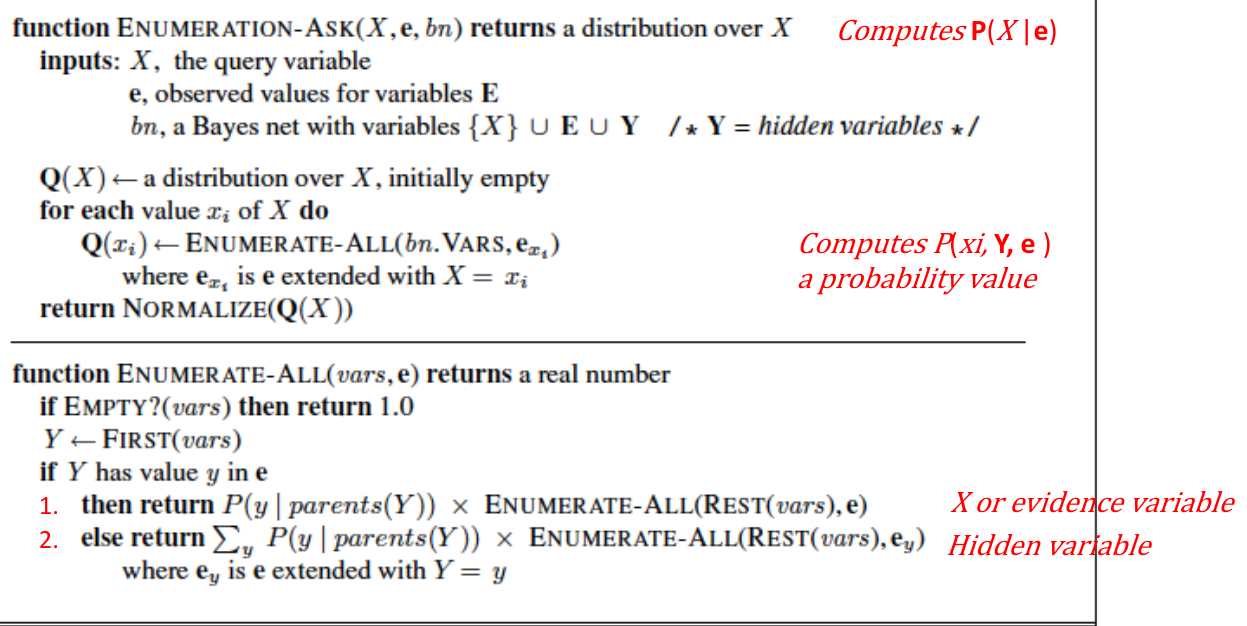
\includegraphics[width=\textwidth]{Images/enumerationAsk}
	\caption{Pseudocode for Enumeration Ask}
	\label{img:enumerationAsk}
\end{figure}
In figure \ref{img:enumerationAsk} there is the pseudocode for the inference procedure 
using enumeration, that can be improved substantially, by storing and reusing the
results of repeated computations (a kind of dynamic programming).\newline
The variable elimination algorithm, proceeds right-to-left (bottom-up) and 
conditional probabilities are represented as factors, matrices resulting from conditional
probabilities and the names make explicit the argument.\newline
For example if we have $P(a | b, e)$ we define the factor $f_i(a, b, e)$ and 
two operations on factors: pointwise-product $(x)$ and summing out variables.

Given a variable and some evidence, a factor can be built by looking at the variable part
of CPTS’s in the network, using $\proc{MAKE-FACTOR(var, e)}$ and the 
\emph{pointwise product} of two factors $f_1$ and $f_2$ yields a new factor $f_3$
such that variables are the union of the variables in $f_1$ and $f_2$ and
elements are given by the product of the corresponding values in the two factors, so
for example computation of the poitnwise product $f_1(A, B) \times f_2(B, C)$ gives
$f_3(A, B, C)$ and the result is not necessarily a probability distribution.

Computational saving comes from the realization that any factor that does not depend
on the variable to be summed out can be moved outside the summation and this operation
of "distributing out" common factors is part of the operation, which in
the general case returns a set of factors.\newline
In figure \ref{img:improvedEliminationAsk} is possible note this improved version of 
variable elimination, where $\proc{MAKE-FACTOR}$ creates a factor for each variable,
given the evidence and $\proc{SUM-OUT}$ sums out over the possible values of a hidden variable,
producing a set of factors; it takes care of distributing out factors 
which do not depend on the variable.

\begin{figure}
	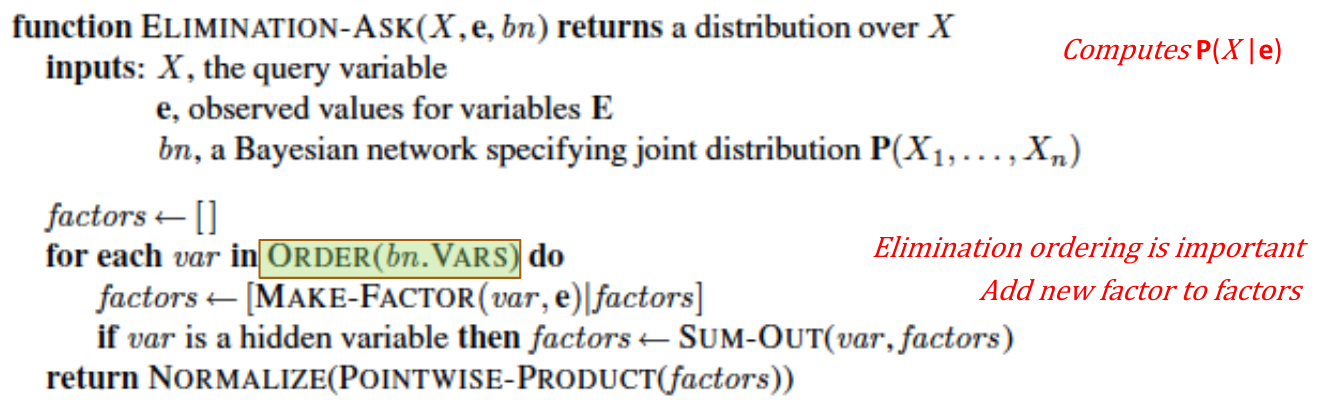
\includegraphics[width=\textwidth]{Images/variableElimination}
	\caption{Pseudocode for Variable elimination algorithm}
	\label{img:improvedEliminationAsk}
\end{figure}
Every choice of ordering yields a valid algorithm, but different orderings of variables
can produce differences in efficiency, but determining the optimal ordering is intractable,
but several good heuristics are available, for example eliminate whichever
variable minimizes the size of the next factor to be constructed.

We can remove any leaf node that is not a query variable or an evidence variable, and 
continuing this process, we can remove any variable that is not an ancestor of a query
variable or evidence variable.

The complexity of exact inference in Bayesian networks depends strongly on the structure
of the network, singly connected networks or polytrees are such that there
is at most one undirected path between any two nodes.\newline
The time and space complexity of exact inference in polytrees is linear in the size
of the network (the number of CPT entries).\newline
For multiply connected networks variable elimination can have exponential time and 
space complexity in the worst case, infact inference in Bayesian networks 
includes as a special case propositional inference, which is NP-complete.

\section{Probabilistic reasoning over time}
So far, we have been doing uncertain reasoning in a static world and for reasoning in an
evolving world an agent needs:
\begin{description}
   \item [belief state: ] the states of the world that are possible.
   \item [transition model: ] to predict how the world will evolve.
   \item [sensor model: ] to update the belief state from perceptions.
\end{description}
A changing world is modeled using a variable for each aspect of the world state at each point
in time (fluents) and we use probabilities to quantify how likely a world is.\newline
The transition and sensor model themselves may be uncertain:
\begin{itemize}
   \item the \emph{transition model} gives the probability distribution of the variables
	 at time $t$, given the state of the world at past times.
   \item the \emph{sensor model} describes the probability of each percept at time $t$,
	 given the current state of the world.
\end{itemize}
We view the world as a series of snapshots, or time slices, each of which contains a set of
random variables, some observable and some not.\newline
$X_t$ will denote the set of state variables, unobservable (hidden) at time $t$ and 
$E_t = e_t$ will denote the set of observations (evidence variables) at time $t$, with 
$e_t$ their values.\newline
We will assume that the state sequence starts at $t=0$ and the distance between time slices 
is fixed and we will use the notation $a:b$ to denote the sequence of integers 
from $a$ to $b$ (inclusive), and the notation $X_{a:b}$ to denote the set of variables
from $X_a$ to $X_b$.

The transition model specifies how the world evolves, the probability distribution over the
latest state variables, given the previous values starting from time $0$
\[ P(X_t | X_{0:t-1}) \]
The sequence of states can become very large, unbounded as $t$ increases and we define the 
\emph{Markov assumptions}: the transition model specifies the probability distribution
over the latest state variables, given a finite fixed number of previous states
\[ P(X_t | X_{0:t-1}) = P(X_t | X_{t-1}) \quad \text{first order Markov chain} \]
\[ P(X_t | X_{0:t-1}) = P(X_t | X_{t-1}, X_{t-2}) \quad \text{second order Markov chain} \]
Additionally, we assume a stationary process, so the conditional probability distribution
is the same for all $t$, since sometimes change is governed by laws that do not themselves
change over time.

\begin{figure}
	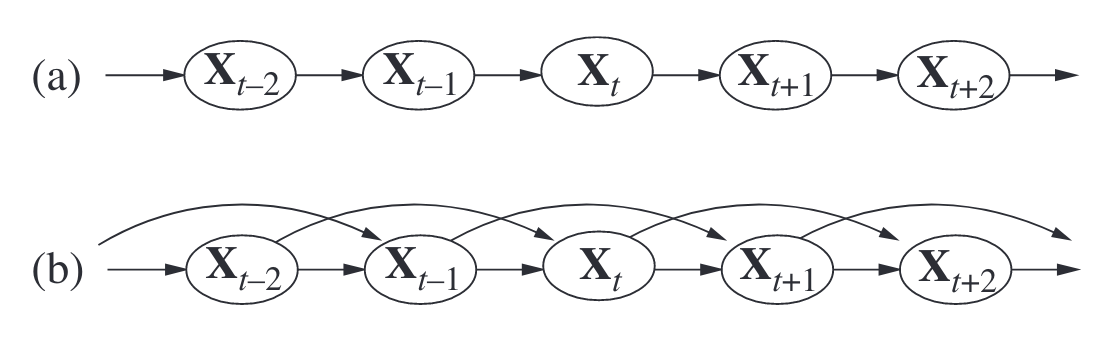
\includegraphics[width=\textwidth]{Images/bayesianMarkov}
	\caption{Bayesian Network of Markov chain}
	\label{img:bayesianMarkov}
\end{figure}
In figure \ref{img:bayesianMarkov} is possible note the transition model using Markov 
chain in Bayes networks and the sensor/observation model, under Markov sensor assumption,
postulates that evidence only depends on the current state
\[ P(E_t | X_{0:t}, E_{0:t-1}) = P(E_t | X_t) \]
This is a reasonable assumption to make, given the availability of sensors.\newline
Assuming for example that "Rain" only depends on rain the previous day may be a too strong
assumption, so there are two ways to improve the accuracy of the approximation:
\begin{enumerate}
    \item Increasing the order of the Markov process model, for example using
	  a second order assumption.
    \item Increasing the set of state variables: we could add Season, Temperature, Humidity,
          Pressure and so on as state variables.\newline
	  This may imply more computation for predicting state variables or adding new sensors.
\end{enumerate}
We also need the prior probability distribution at time $0, P(X_0)$, so putting all together,
the complete joint distribution over all the variables, for any $t$, 
computed from the network is
\[ P(X_{0:t}, E_{1:t}) = P(X_0) \prod _{i=1}^t P(X_i | X_{i-1}) P(E_i | X_i) \]

Basic inference tasks based on the temporal model, consist in the following operations:
\begin{description}
   \item [Filtering:]  computing the belief state (posterior probability distribution of 
	   state variables) given evidence from previous and current states.\newline
	   A subtask is the likelihood of the evidence sequence $P(X_t | e_{1:t})$.
   \item [Prediction: ] computing the posterior distribution over a future state, given all
          evidence to date, so we compute $P(X_{t+k} | e_{1:t})$ with $k > 1$.
   \item [Smoothing: ] computing the posterior distribution over a past state, given all
	   evidence up to the present.\newline
	   Looking back with the knowledge of today provides a more accurate estimate, so
	   we have $P(X_k |e_{1:t})$ with $0 \leq  k < t$.
   \item [Most likely explanation/sequence: ] given a sequence of observations, we might wish
       to find the sequence of states that is most likely to have generated those observations.
   \item [Learning: ] the transition and sensor models, can be learned from observations.
\end{description}
\begin{figure}
	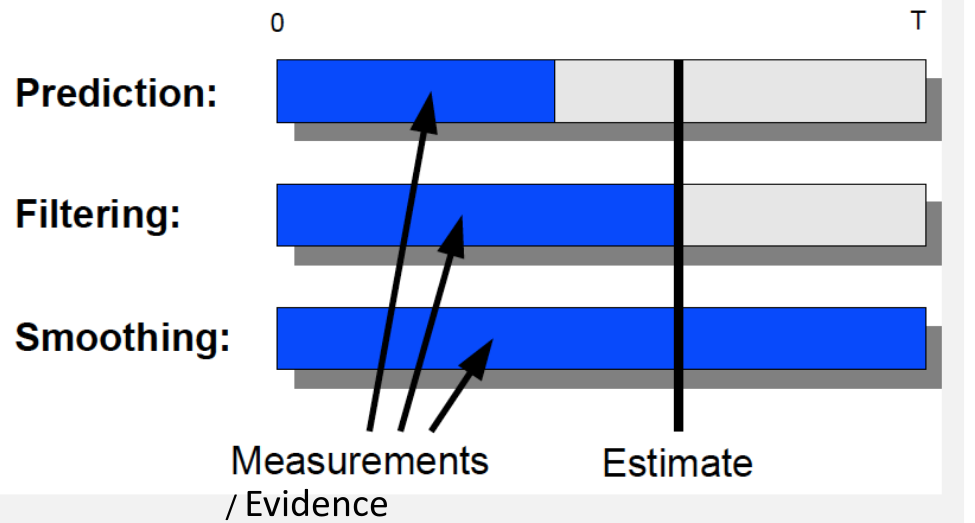
\includegraphics[width=\textwidth]{Images/inferenceOperations}
	\caption{Interaction between time and inference operations}
	\label{img:filtering}
\end{figure}
In figure \ref{img:filtering} is possible to note how some inference operations interface
with past, current and future state and a good filtering algorithm maintains a current state
estimate and updates it, rather than going back over the entire history of percepts
for each time.\newline
The filtering function $f$ takes into account the state estimation computed up to the
present and the new evidence.
\[ P(X_{t+1} | e_{1:t+1}) = f(e_{t+1}, P(X_t | e_{1:t}) \]
This process is called \emph{recursive estimation} and is made of two parts:
\begin{description}
   \item [Prediction: ] the current state distribution is projected forward from $t$ to $t+1$:
	   \[ P(X_{t+1} | e_{1:t}) \]
   \item [Update: ] it is updated using the new evidence $e_{t+1} P(e_{t+1} | X_{t+1})$.
\end{description}
Filtering can be computed as follows:
\begin{align*}
    P(X_{t+1} | e_{1:t+1}) & = P(X_{t+1} | e_{1:t}, e_{t+1}) \\
	                   & = \alpha P(e_{t+1} | X_{t+1}, e_{1:t}) P(X_{t+1} | e_{1:t}) \\
			   & = \alpha P(e_{t+1} | X_{t+1}) P(X_{t+1} | e_{1:t}) \\
			   & = \alpha P(e_{t+1} | X_{t+1}) \sum_{x_t} P(X_{t+1}| x_t, e_{1:t})
			                                               P(x_t | e_{1:t}) \\
			   & = \alpha P(e_{t+1}|X_{t+1}) \sum_{x_t} P(X_{t+1} | x_t) 
			                                            P(x_t | e_{1:t}) \\
\end{align*}
We can think of $P(X_t|e_{1:t})$ as a message $f_{1:t}$ that is propagated forward
in the sequence and this makes evident the recursive structure:
\[ f_0 = P(X_0) \]
\[ f_{1:t+1} = \alpha Forward(f_{1:t}, e_{t+1}) \]
where $Forward$ implements the filtering update in constant time.

The task of prediction can be seen simply as filtering without the contribution of new
evidence and also the filtering process already incorporates a one-step prediction.\newline
In general, looking ahead $k$ steps, at time $t+k+1$, given evidence up to $t$ is done by
\[ P(X_{t+k+1} | e_{1:t}) = \sum _{x_{t+k}} P(X_{t+k+1} | x_{t+k}) P(x_{t+k} | e_{1:t}) \]
This computation involves only the transition model and not the sensor model and 
we can show that the predicted distribution for Rain converges to a fixed point $(0.5, 0.5)$,
after which it remains constant for all time (the stationary distribution of the
Markov process).\newline
The \emph{mixing time} is the time to reach the fixed point and we have that the more
uncertainty there is in the transition model, the shorter will be the mixing time
and the more the future is obscure.

We can use a forward recursion also to compute the likelihood of an evidence sequence
P e 1:t , useful if we want to compare two models producing the same evidence sequence.\newline
We can derive a recursive equation similar to filtering and a similar likelihood message
\[ l_{1:t}(X_t) = P(X_t, e_{1:t}) \]
Once we have $l_{1:t}(X_t)$ we can compute the likelihood of the evidence sequence by
summing out on the values of $X_t$ as follows
\[ L_{1:t} = P(e_{1:t}) = \sum _{x_t} l_{1:t}(x_t) \]
Note that the likelihood becomes smaller and smaller as $t$ increases.

Smoothing is the process of computing the posterior distribution of the state at some
past time $k$ given a complete sequence of observations up to the present $t$
\[ P(X_k | e_{1:t}) \quad \text{for } 0 \leq k < t \]
The additional evidence is expected to provide more information and more accurate
predictions on the past.

To compute the smoothing we have the following phases
\begin{align*}
   P(X_k | e_{1:t}) & = P(X_k | e_{1:k}, e_{k+1:t}) \\
	            & = \alpha P(X_k | e_{1:k}) P(e_{k+1:t} | X_k, e_{1:k}) \\
		    & = \alpha P(X_k | e_{1:k}) P(e_{k+1:t} | X_k) \\
		    & = \alpha f_{1:k} \times b_{k+1:t} \\
\end{align*}
$P(X_k|e_{1:k})$ corresponds to the forward message $f_{1:k}$, computed up to $t$,
as before in filtering and we define another message $b_{k+1:t} = P(e_{k+1:t}|X_k)$ 
that can be computed by a recursive process that runs backward from $t$.\newline
The terms in $f_{1:k}$ and $b_{k+1:t}$ can be implemented by two recursive calls,
one running forward from $1$ to $k$ and using the filtering equation and 
the other running backward from $t$ to $k+1$ for computing $P(e_{k+1:t}|X_k)$.

To compute smoothing going backwards we have 
\begin{align*}
   P(e_{k+1:t} | X_k) & = \sum _{x_{k+1}} P(e_{k+1:t}|X_k, x_k+1) P(x_{k+1}|X_k) \\
	              & = \sum _{x_{k+1}} P(e_{k+1:t}|x_{k+1}) P(x_{k+1}|X_k) \\
		      & = \sum _{x_{k+1}} P(e_{k+1}, e_{k+2:t} | x_{k+1}) P(x_{k+1} | X_k) \\
		      & = \sum _{x_{k+1}} P(e_{k+1} | x_{k+1}) P(e_{k+2:t} | x_{k+1})
		                          P(x_{k+1} | X_k) \\
\end{align*}
$b_{k+1:t} = P(e_{k+2:t}|x_{k+1})$ is defined by the previous equation computing backward
and the backward phases start with $b_{t+1:t} = 1$ and then we compute 
\[ b_{k+1:t} = Backward(b_{k+2:t}, e_{k+1}) \]
where $Backward$ implements the update defined above.

To improve efficincy we use an algorithm, called \emph{forward–backward}, visible in figure
\ref{img:forwardBackward}, which uses dynamic programming to reduce the complexity
of running the algorithm over the whole sequence.\newline
The trick is to record the results computed during the forward filtering phase,
over the whole sequence, and reuse them during the backward phase, so we obtain that 
the complexity is $O(t)$ and is consistent with the fact that the 
Bayesian network structure is a polytree.\newline
The forward–backward algorithm is the basis for many applications that deal
with sequences of noisy observations and improvements are required to deal with
space complexity for long sequences and online computations, where new observations
continuously arrive (fixed-lag smoothing).

\begin{figure}
	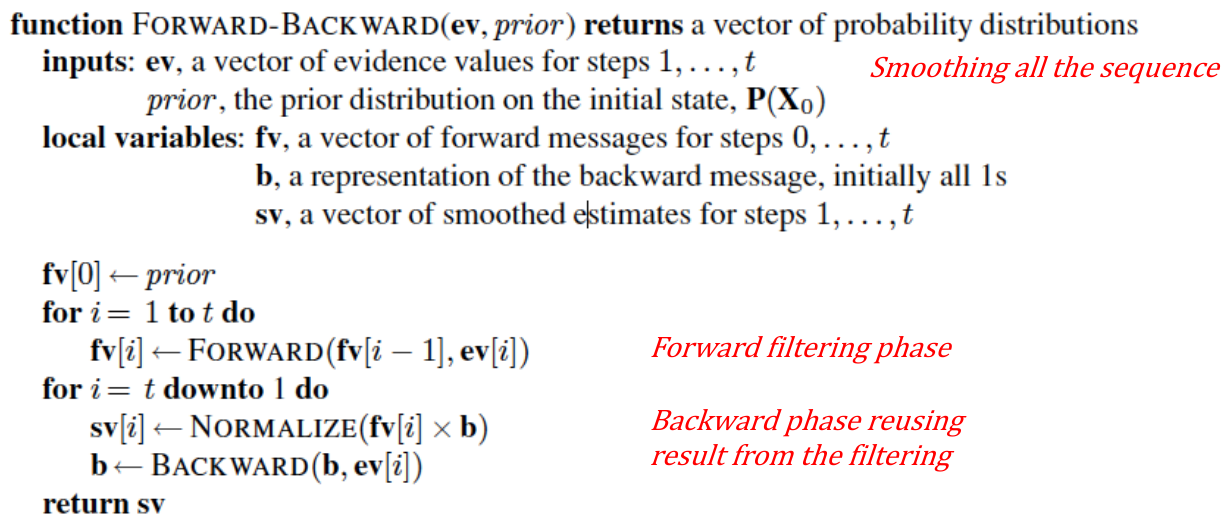
\includegraphics[width=\textwidth]{Images/forwardBackward}
	\caption{Pseudocode for ForwardBackward algorithm}
	\label{img:forwardBackward}
\end{figure}
Suppose we observe [ true, true, false, true, true ] for the Umbrella variable, so 
what is the most likely sequence for Rain given these oservations?\newline
There are $2^5$ possible Rain sequences, and each sequence is a path through a graph
whose nodes are the possible states at each time step.\newline
We want to discover which is the one maximizing the likelihood, in linear time and the 
likelihood of a path is the product of the transition probabilities along the path and
the probabilities of the given observations at each state.

There is a recursive relationship between the most likely path to each state $x_{t+1}$ 
and most likely paths to each previous state $x_t$.\newline
We can write a recursive equation, similar to the one for filtering as 
\[ \max_{x_1, \dots, x_t} P(x_1, \dots, x_t, X_{t+1} | e_{1:t+1}) = 
   \alpha P(e_{t+1} | X_{t+1}) \max_{x_t} (P(X_{t+1}|X_t) \max_{x_1, \dots, x_{t-1}}
   P(x_1, \dots, x_{t-1}, x_t | e_{1:t})) \]
The forward message in this case is $\max P(x_1, \dots, x_{t-1}, X_t | e_{1:t})$,
the probabilities of the best path to each state $x_t$; from those we can compute
the probabilities of the extended paths at time $t+1$ and take the max.\newline
The most likely sequence overall can be computed in one pass and for each state,
the best state that leads to it is recorded (marked as black arrows in the example)
so that the optimal sequence is identified by following black arrows backwards from the best
final state.\newline
This algorithm is the famous \emph{Viterbi algorithm}, named after A. Viterbi [1967]

The original application of Viterbi was in telecommunications: Viterbi decoders are used
for decoding a bitstream encoded using a technique called convolutional code or trellis code,
but is also used in NLP as different kinds of "sequence tagger" or also Speech recognition
(speech-to-text), speech synthesis, speech diarization.

We now present an overview of other approaches:
Probability theory and Bayesian networks are the dominant approaches today, despite
the disadvantage of having to specify many probability values (lots of numbers), so
other approaches are used to help humans to understand reasoning behind:
\begin{enumerate}
    \item Rule-based methods for uncertain reasoning in expert systems.
    \item Representing ignorance: Dempster–Shafer theory.
    \item Representing vagueness: fuzzy sets and fuzzy logic.
\end{enumerate}
Three good properties of classical logic-based rules:
\begin{description}
    \item [Locality: ] In logical systems, from $A$ and $A \to B$, we can conclude $B$,
	              without worrying about any other rules, instead in probabilistic systems,                      we need to consider all the evidence.
   \item [Detachment: ] once $B$ is proved, it can be used regardless of how it was derived and
	               it can be detached from its justification.
   \item [Truth-functionality: ] the truth of complex sentences can be computed from the
	          truth of the components, instead probability combination
		  does not work this way.
\end{description}
In Rule-based methods the idea is to attach degree of belief to facts and rules and 
to combine and propagate them, and the most famous example is the certainty factors model,
which was developed for the MYCIN medical diagnosis program.\newline
The system was carefully engineered to avoid mixing different kind of rules 
(diagnostic vs causal), trying to control non plausible results.

The theory of \emph{fuzzy sets} is a way to specify how well an object satisfies a vague
description (non categorical) property, like "being tall".\newline
Fuzziness is not uncertainty in the world, but is the uncertainty
in the use of qualifiers/properties.\newline
Fuzzy logic is way of reasoning about membership in fuzzy sets and a fuzzy predicate
implicitly defines a fuzzy set.\newline
Fuzzy logic is a method for reasoning with logical expressions describing
membership in fuzzy sets and standard rules used are 
\[ T(A \land B) = \min (T(A), T(B)) \]
\[ T(A \lor B) = \max (T(A), T(B)) \]
\[ T(\neg A) = 1 - T(A) \]

Fuzzy control is a methodology for constructing control systems in which the mapping
between real-valued input and output parameters is represented by fuzzy rules.\newline
It consist on the following operations:
\begin{description}
    \item [Fuzzification: ] continous variables are mapped into a set of linguistic variables
	    with fuzzy values; temperature can be mapped in fuzzy variables such as 
	    low, medium, high and their membership functions.
    \item [Reasoning: ] with rules expressed in terms of these fuzzy variables,
	    reaching fuzzy conclusions.
    \item [Defuzzification: ] map the results into numerical valueo far,
	   we have been doing uncertain reasoning in a static world.
\end{description}
